% Overleaf: upload this file together with the microscopy_figures/ directory.
% The supplied microscopy_overleaf.zip contains the complete upload bundle.
% Main document: microscopy_analysis_report.tex; compiler: pdfLaTeX.
% References are embedded. No raw TIFF, notebook execution, or shell escape is needed.
\documentclass[11pt,letterpaper]{article}
\usepackage[T1]{fontenc}
\usepackage[utf8]{inputenc}
\usepackage{lmodern}
\usepackage[margin=0.9in]{geometry}
\usepackage{microtype}
\usepackage{amsmath,amssymb}
\usepackage{graphicx}
\usepackage{booktabs,longtable,tabularx,array}
\usepackage{enumitem,needspace}
\usepackage{xcolor}
\usepackage{xurl}
\usepackage{listings}
\usepackage{fancyhdr}
\usepackage{pdflscape}
\usepackage[section]{placeins}
\definecolor{navy}{HTML}{17365D}
\definecolor{teal}{HTML}{216869}
\definecolor{lightblue}{HTML}{F0F5F8}
\usepackage[colorlinks=true,linkcolor=navy,citecolor=teal,urlcolor=teal,
  pdftitle={Microscopy: From Intensity Inspection to Segmented Objects},
  pdfauthor={LEC2026 Faculty AI Workshop}]{hyperref}
\graphicspath{{microscopy_figures/}{workshop/reports/microscopy_figures/}}
\newcolumntype{L}[1]{>{\raggedright\arraybackslash}p{#1}}
\newcolumntype{Y}{>{\raggedright\arraybackslash}X}
\newcommand{\field}[1]{\nolinkurl{#1}}
\newcommand{\px}{\ensuremath{\mathrm{px}}}
\newcommand{\pxsq}{\ensuremath{\mathrm{px}^{2}}}
\newcommand{\notebookfig}{\textbf{Saved notebook figure.}}
\newcommand{\diagnosticfig}{\textbf{Supplemental diagnostic.}}
\setlength{\parskip}{5pt}
\setlength{\parindent}{0pt}
\setlength{\headheight}{14pt}
\setlength{\emergencystretch}{2em}
\renewcommand{\arraystretch}{1.16}
\setlist[itemize]{topsep=3pt,itemsep=2pt}
\setlist[enumerate]{topsep=3pt,itemsep=3pt}
\setcounter{tocdepth}{1}
\pagestyle{fancy}
\fancyhf{}
\fancyhead[L]{\small Microscopy: an explained analysis workflow}
\fancyhead[R]{\small LEC2026}
\fancyfoot[C]{\thepage}
\lstset{basicstyle=\ttfamily\footnotesize,breaklines=true,
  columns=fullflexible,keepspaces=true,showstringspaces=false,
  frame=single,rulecolor=\color{lightblue},backgroundcolor=\color{lightblue},
  xleftmargin=3pt,xrightmargin=3pt,aboveskip=8pt,belowskip=8pt}

\title{\textbf{Microscopy: From Intensity Inspection\\to Segmented Objects}\\[7pt]
  \large An Illustrated, Step-by-Step Explanation of the Notebook}
\author{LEC2026 Faculty AI Workshop}
\date{October 24, 2026}

\begin{document}
\maketitle
\thispagestyle{empty}
\begin{abstract}
This report explains the microscopy notebook as a sequence of explicit decisions: inspect pixel intensities, smooth local fluctuations, choose a global threshold, clean a foreground mask, identify object centres, partition touching structures, measure the resulting regions, and evaluate parameter sensitivity. All five plots saved in the notebook are reproduced unchanged. Seven additional diagnostic figures expose intermediate arrays that the notebook computes but does not display, or clarify a display/selection choice.

The input is one $512\times512$ grayscale microscopy field from scikit-image's \field{human_mitosis} example. With the saved default settings, the analysis returns 297 segmented objects, including 26 touching the image border. These are algorithm-defined image regions. A biological cell count, mitotic index, physical area in square micrometres, or segmentation accuracy would require information and validation beyond this example. The purpose is to make the computation understandable and reviewable, including its assumptions, limitations, and the reasons a visually plausible result may still need scientific correction.
\end{abstract}

\begin{center}\small
\begin{tabular}{ll}
\toprule
\textbf{Companion notebook} & \field{03_microscopy.ipynb} \\
\textbf{Image} & \field{mitosis.tif}; 512 rows $\times$ 512 columns; unsigned 8-bit \\
\textbf{Observed intensity range} & 7--255; median 10 \\
\textbf{Default segmentation} & Threshold factor 1.0; minimum area 40\,\pxsq; seed spacing 8\,\px \\
\textbf{Default result} & 297 objects; median area 89\,\pxsq; 26 edge-touching objects \\
\textbf{Figures} & Five saved notebook plots and seven labelled diagnostics \\
\bottomrule
\end{tabular}
\end{center}
\clearpage
\tableofcontents
\clearpage

\section{What the notebook is trying to accomplish}

The notebook turns a grayscale image into a labelled image and a table of region measurements. A grayscale image describes intensity at each pixel. A binary mask decides which pixels belong to the candidate foreground. A labelled image goes further: each surviving object receives an integer identifier, allowing the software to measure it separately.

The scientific question is deliberately narrow: \emph{how do thresholding, mask cleanup, and watershed seeds affect the bright regions that we identify and measure in this field?} The educational question is how faculty can use a transparent analysis function, modify one choice at a time, and check the result against the source image.

The source is scikit-image's \field{human_mitosis} field, attributed to David Root and released under CC0. The data documentation associates it with Moffat and colleagues' work on human cells.\cite{data} The kit does not provide the staining/acquisition metadata needed to assign every bright structure a specific identity, a reference segmentation mask, or pixel-size calibration. The report therefore uses \emph{bright structures}, \emph{regions}, and \emph{segmented objects} for the algorithm's outputs.

The first meaningful analytical action is to inspect intensity. Everything that follows depends on whether intensity provides a useful starting distinction between foreground and background.

\section{Step 1: inspect the image and its intensity distribution}
\label{sec:intensity}

\subsection{Check the array before interpreting the picture}
The loader verifies the source-file checksum, checks that the array has shape $(512,512)$, and checks that its data type is \field{uint8}. These checks protect against analysing a different file, an unexpected colour image, or a different numerical representation. The checksum identifies the bytes of the input, not its biological correctness.

There are $512\times512=262{,}144$ pixels. Unsigned 8-bit storage permits integer values from 0 to 255, but the observed minimum in this image is 7. The observed maximum is 255. A nonzero background is entirely compatible with an image of bright structures on a dark field: the background does not have to be numerically zero.

The initial code prints the intensity range and draws the original image next to a histogram:
\begin{lstlisting}[language=Python]
axes[0].imshow(image, cmap="gray", vmin=0, vmax=255)
axes[1].hist(image.ravel(), bins=64)
axes[1].set(yscale="log")
\end{lstlisting}
\field{image.ravel()} lists all pixels in one dimension for counting. It changes the view used for the histogram, not the intensities or their positions in the source array.

\begin{figure}[htbp]
\centering
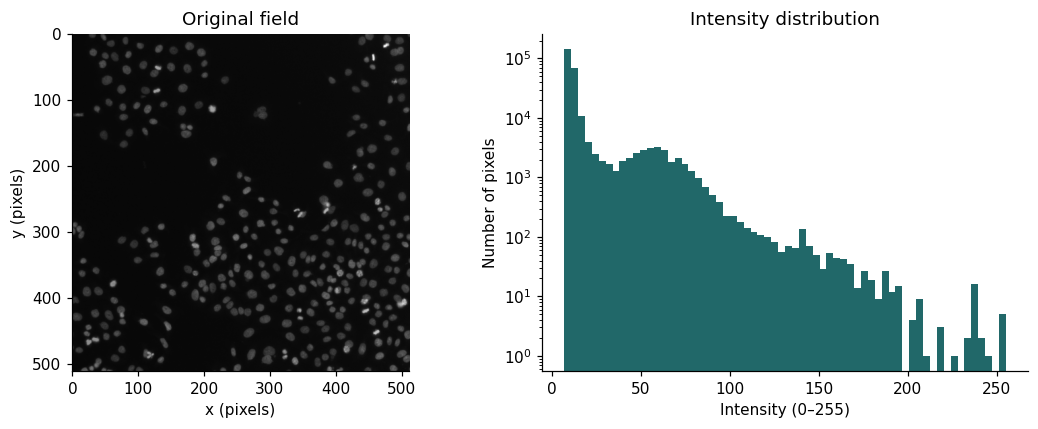
\includegraphics[width=\linewidth]{01_notebook_intensity.png}
\caption{\notebookfig\ Original field and intensity histogram, extracted from the notebook's first image-inspection plot. The image uses a fixed display range of 0--255. The histogram counts pixels in 64 bins and uses a logarithmic vertical axis.}
\label{fig:intensity}
\end{figure}

\subsection{Read the two panels together}
The left panel shows spatial structure. Bright objects are concentrated in some parts of the field, and a large central area is relatively dark. The histogram discards that spatial arrangement and answers a different question: how many pixels have intensities in each range?

The strong low-intensity peak is consistent with a field dominated by background. A smaller population of brighter pixels forms a shoulder and a long tail. This pattern motivates an intensity-based foreground mask. It does not prove that every bright pixel is biological foreground or that every biologically relevant structure is bright enough to be retained.

The logarithmic count axis is essential to reading the plot. Moving from $10^{2}$ to $10^{3}$ means ten times as many pixels, rather than 100 additional pixels. It reveals relatively rare bright intensities that would be difficult to see on a linear count scale. It does not transform the image intensities supplied to the segmentation algorithm.

The 64 histogram bins group nearby intensity values, approximately four integer levels per bin over the observed range. This is an exploratory display. As explained in Section~\ref{sec:otsu}, the actual Otsu calculation uses a different histogram: 256 bins of the \emph{smoothed floating-point image}.

\begin{table}[htbp]
\centering
\caption{Descriptive checks on the unchanged input image. Percentiles describe pixel values, not independent biological samples.}
\begin{tabular}{lr}
\toprule
\textbf{Quantity} & \textbf{Value} \\
\midrule
Pixels & 262,144 \\
Minimum / median / maximum & 7 / 10 / 255 \\
Mean intensity & 17.2945 \\
25th / 75th percentile & 9 / 13 \\
95th / 99th percentile & 63 / 91 \\
Pixels at the maximum stored value 255 & 2 \\
\bottomrule
\end{tabular}
\end{table}

Only two pixels are at 255. That is a useful clipping check, but these values alone do not establish detector saturation: the original acquisition and any previous scaling are not fully documented in this kit. Similarly, raw intensity is not automatically a concentration, molecule count, or calibrated fluorescence measurement.

\subsection{What should be checked at this stage?}
Before choosing a threshold, ask whether the image has usable contrast, substantial spatial variation in background, obvious clipping, or structures that overlap in intensity with their surroundings. A single global threshold may struggle with uneven illumination or dim structures. The notebook does not first estimate and subtract a background image; its later threshold should be interpreted with that limitation in mind.

\section{A display check: brightness on the page is not the measurement}
\label{sec:display}

\field{imshow} maps numerical values to display shades. In the full-field plot, specifying \field{vmin=0, vmax=255} fixes this mapping. A value of 100 receives the same shade whenever those limits are used.

The notebook's later crop uses \field{imshow(crop, cmap="gray")} without fixed limits. That crop has observed intensities 7--108, so the display maps this narrower interval across the grayscale range. Its structures consequently look brighter and higher-contrast than they do in a fixed 0--255 display, despite having the same pixel values.

\begin{figure}[htbp]
\centering
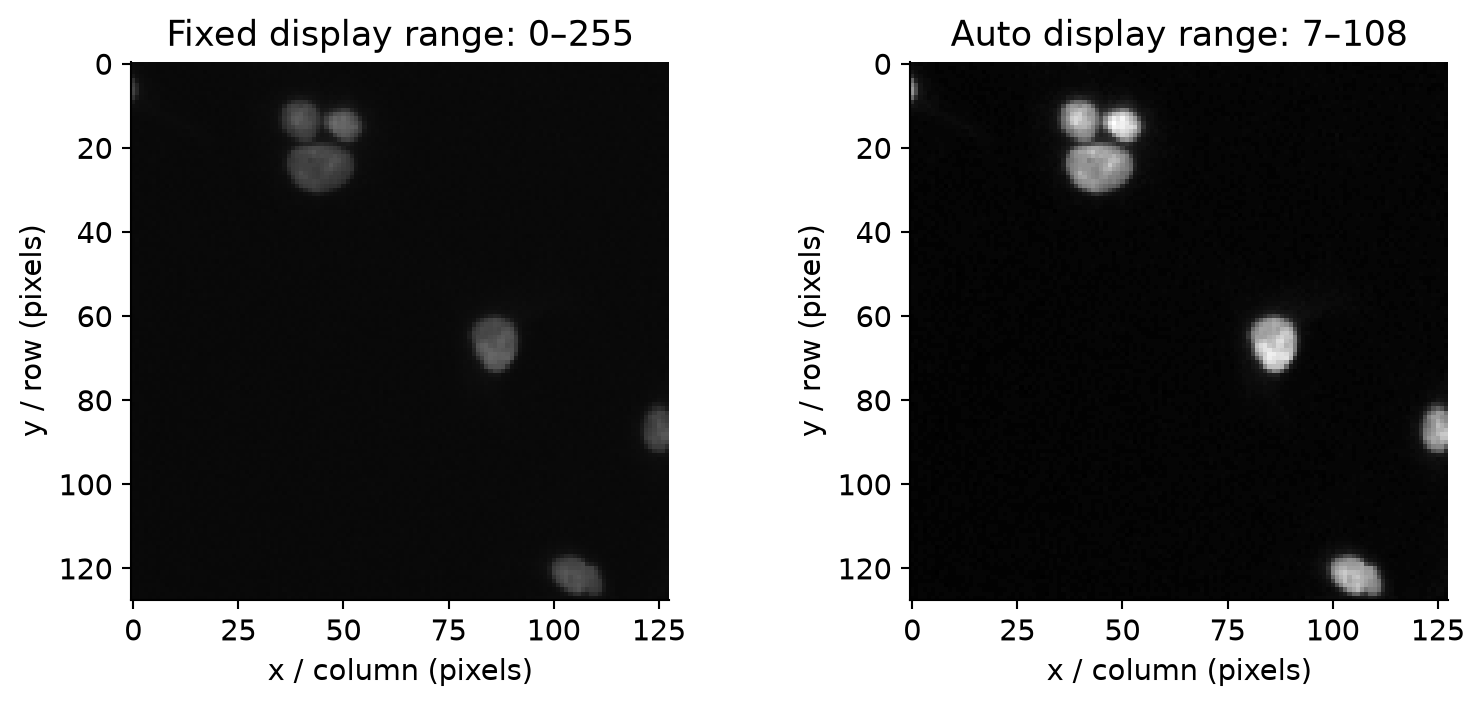
\includegraphics[width=\linewidth]{06_display_scaling.png}
\caption{\diagnosticfig\ Exactly the same original 128-by-128 crop shown with fixed 0--255 limits and with the crop's automatic 7--108 limits. This is a display comparison, not an image-processing step in the segmentation.}
\label{fig:display}
\end{figure}

This distinction matters when judging improvements. A brighter-looking panel may reflect a different display mapping, not a better signal, a changed measurement, or a more accurate segmentation. Comparing filtering effects is easier when the before and after images share the same display limits.

\section{Step 2: smooth local fluctuations with a Gaussian filter}
\label{sec:gaussian}

\subsection{What the code does}
The function begins with:
\begin{lstlisting}[language=Python]
smoothed = filters.gaussian(image, sigma=1.0, preserve_range=True)
\end{lstlisting}
The Gaussian filter replaces each pixel by a weighted local average, with greater weight given to nearby pixels. Its two-dimensional weighting function has the form
\begin{equation}
G_{\sigma}(u,v)=\frac{1}{2\pi\sigma^{2}}
\exp\left[-\frac{u^{2}+v^{2}}{2\sigma^{2}}\right],
\qquad J=G_{\sigma}*I,
\end{equation}
where $I$ is the original image and $J$ is the smoothed image. The discrete implementation normalizes sampled weights; the equation expresses the weighting principle.

Here $\sigma=1$ pixel along both image axes. It is a spatial scale in pixels, not micrometres. In the documented defaults, the kernel is truncated at four standard deviations, giving a radius of four pixels and nine sampled positions along each axis. The default \field{mode='nearest'} extends the nearest edge value beyond the array when a neighbourhood reaches outside the image.\cite{filters,gaussian}

\subsection{Why smooth before thresholding?}
Small local fluctuations can create jagged boundaries, isolated foreground pixels, or unstable threshold crossings. A modest blur reduces that fine-scale variability. It also blends neighbouring values: an isolated high pixel becomes less extreme, edges become softer, and close structures may acquire a bridge. The filter does not distinguish noise from a genuine small feature, so a larger $\sigma$ can remove useful structure as well as fluctuations.

\field{preserve_range=True} retains the original numerical intensity scale rather than converting the 8-bit values to a normalized 0--1 scale. The result is floating point, so values can be fractional. In this reconstruction, the smoothed minimum and maximum are approximately 7.452 and 225.234, rather than 7 and 255. Range preservation means the original scale is retained; it does not mean that local extrema remain unchanged.

\begin{figure}[htbp]
\centering
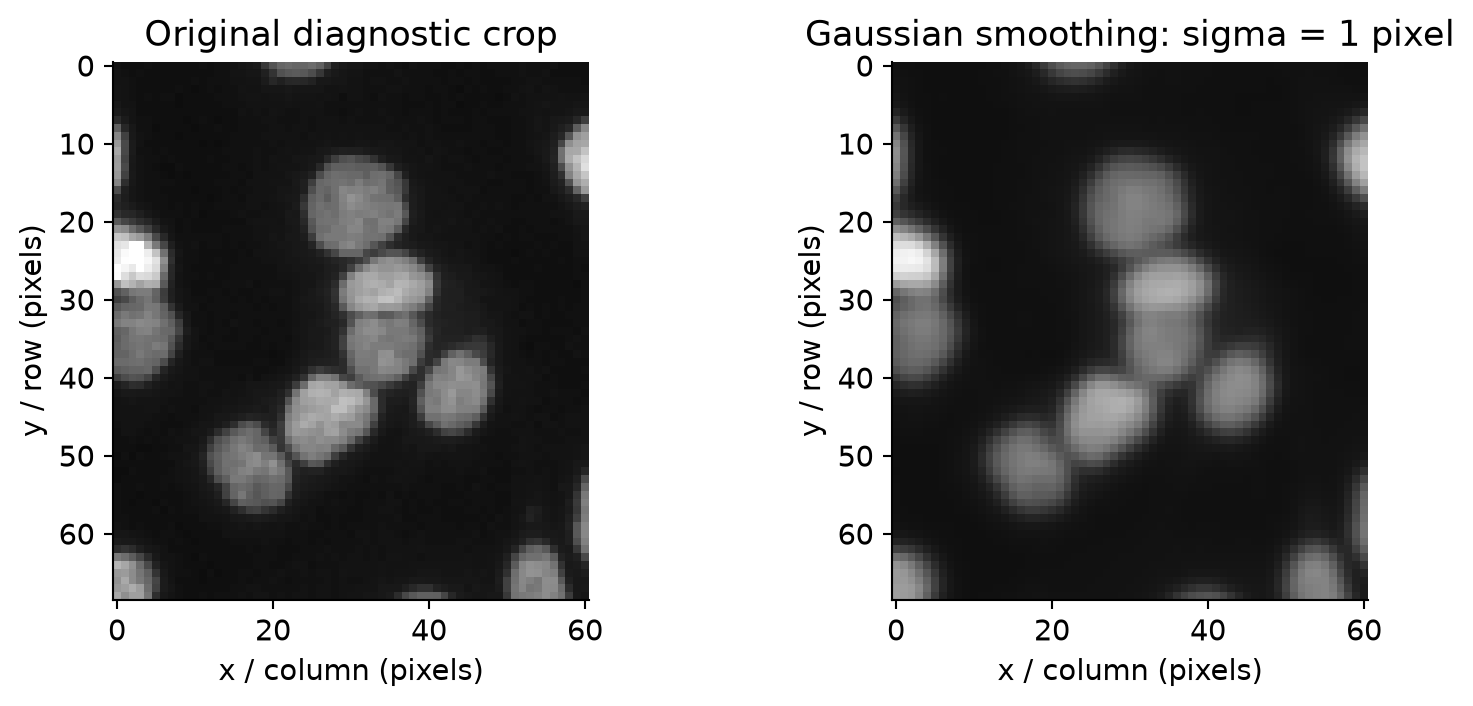
\includegraphics[width=\linewidth]{07_gaussian_comparison.png}
\caption{\diagnosticfig\ The original and Gaussian-smoothed image in a diagnostic crop, using identical grayscale limits. Full-image rows 297--365 and columns 186--246 are shown with local crop coordinates. Fine texture and edges soften; spatial structure remains visible.}
\label{fig:gaussian}
\end{figure}

This Gaussian operation is the notebook's explicit intensity-smoothing filter. The later area filter and hole filling operate on masks or labels, and the distance transform changes the meaning of pixel values entirely. They should not all be described as interchangeable forms of denoising.

\section{Step 3: choose an Otsu threshold and build a binary mask}
\label{sec:otsu}

\subsection{Otsu's statistical criterion}
The notebook computes a single threshold for the smoothed image:
\begin{lstlisting}[language=Python]
threshold = float(filters.threshold_otsu(smoothed)) * threshold_factor
mask = smoothed > threshold
\end{lstlisting}
Otsu's method considers splits of the intensity histogram into a lower-intensity class and a higher-intensity class. It chooses the split maximizing between-class variance, equivalently minimizing weighted within-class variance for the two-class partition.\cite{filters} A useful expression is
\begin{equation}
\tau_{\mathrm{Otsu}}
=\underset{\tau}{\operatorname{arg\,max}}\;
\omega_{0}(\tau)\,\omega_{1}(\tau)
\left[\mu_{0}(\tau)-\mu_{1}(\tau)\right]^{2},
\end{equation}
where $\omega_k$ is the fraction of pixels in class $k$ and $\mu_k$ is its mean intensity. This is a histogram-separation rule. It does not use a biological annotation or learn what a cell is.

The input is the smoothed floating-point array, so the default \field{nbins=256} applies. The method uses one global cutoff across the whole field; it is not an adaptive threshold chosen separately in each neighbourhood.

\subsection{The threshold factor and the strict comparison}
For this image, the default Otsu value is
\[
\tau_{\mathrm{Otsu}}=35.95063855194327.
\]
The tool multiplies it by a user-chosen factor $\alpha$:
\begin{equation}
M_{0}(r,c)=\mathbf{1}\{J(r,c)>\alpha\tau_{\mathrm{Otsu}}\}.
\label{eq:mask}
\end{equation}
At the default $\alpha=1$, the printed value is rounded to 36.0, but the computation uses the full floating-point value. The comparison is strictly greater than the threshold. A pixel equal to the cutoff is not included.

\begin{figure}[htbp]
\centering
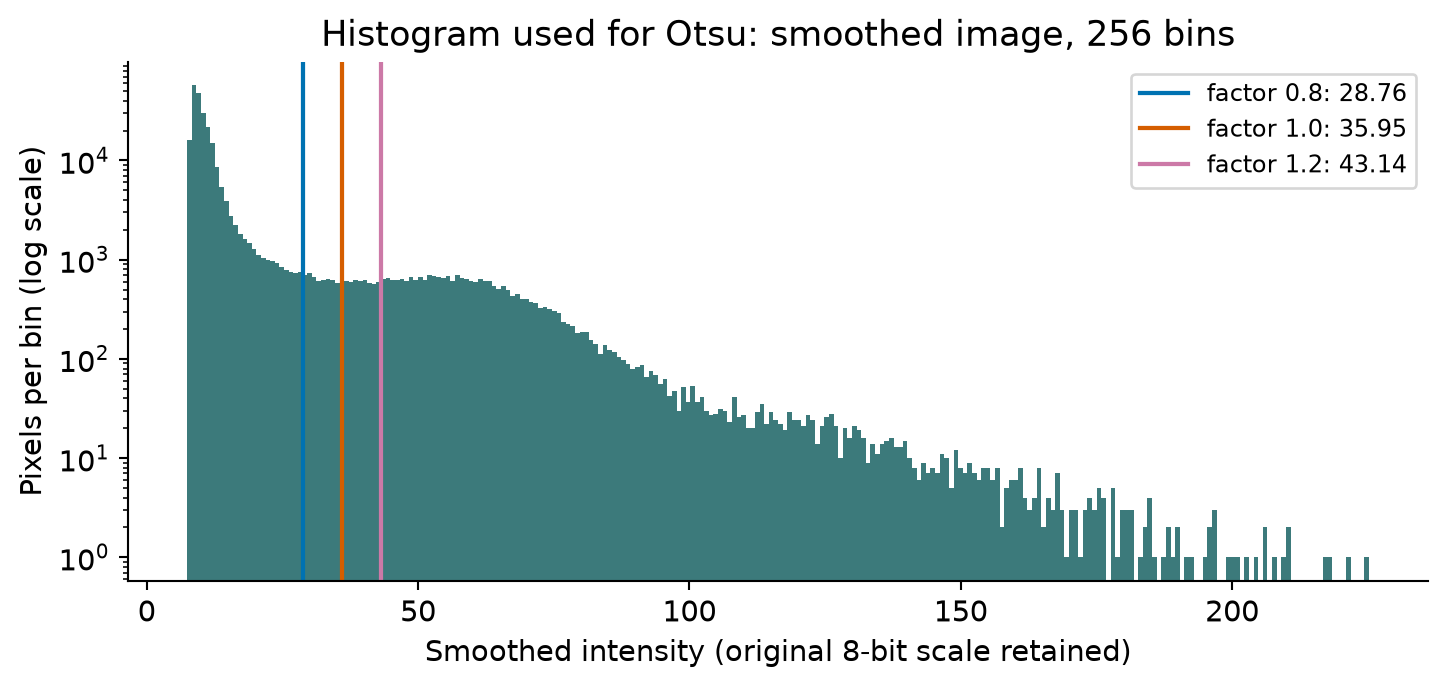
\includegraphics[width=\linewidth]{08_otsu_histogram.png}
\caption{\diagnosticfig\ The smoothed-image histogram with 256 bins, matching the input and bin count used by Otsu. Lines show the scaled cutoffs for factors 0.8, 1.0, and 1.2. The count axis is logarithmic.}
\label{fig:otsu}
\end{figure}

At this point, the output is Boolean: True marks candidate foreground and False marks background. The default threshold selects 31,071 pixels. They do not yet have individual object identities. A continuous white patch can contain several touching structures, and one biological structure can have several disconnected bright patches.

Increasing $\alpha$ reduces or preserves the size of this \emph{initial threshold mask} for a fixed smoothed image. It does not guarantee fewer final objects: changing a bridge or removing a weak region can alter component topology, seed detection, and subsequent splitting. Section~\ref{sec:sensitivity} shows this distinction in the saved results.

\section{Step 4: label connected components and remove small ones}
\label{sec:components}

\subsection{A connected component is a pixel-defined region}
The threshold mask is labelled with:
\begin{lstlisting}[language=Python]
connected = measure.label(mask)
sizes = np.bincount(connected.ravel())
keep = sizes >= int(min_area)
keep[0] = False
mask = keep[connected]
\end{lstlisting}
In this two-dimensional call, \field{measure.label} uses full connectivity by default: pixels touching along an edge \emph{or a corner} can belong to the same component. This is eight-neighbour connectivity. Zero is the background label.\cite{measure}

\field{np.bincount} counts how many pixels have each integer label. The result is an area in pixels. For example, an isolated component containing 12 foreground pixels has area 12\,\pxsq, regardless of its brightness. With \field{min_area=40}, a component survives if it contains \emph{at least} 40 pixels; a component of exactly 40 is retained.

The explicit \field{keep[0]=False} prevents the large background region from being retained merely because it exceeds the size cutoff. Indexing \field{keep[connected]} converts the component-level decisions back into a Boolean pixel mask.

\subsection{What changes in the default result?}
There are initially 276 eight-connected threshold components. Seven are smaller than 40 pixels. Removing them discards 59 foreground pixels and leaves 269 components containing 31,012 pixels in total. This is a small numerical change, which is why the full-field before/after masks look similar.

An area filter is a morphological selection criterion, not a second intensity threshold. A small bright object can be removed, while a larger dimmer component that passed the first threshold can survive. Whether the removed components are debris, legitimate small structures, or edge fragments cannot be decided from their area alone.

\begin{figure}[htbp]
\centering
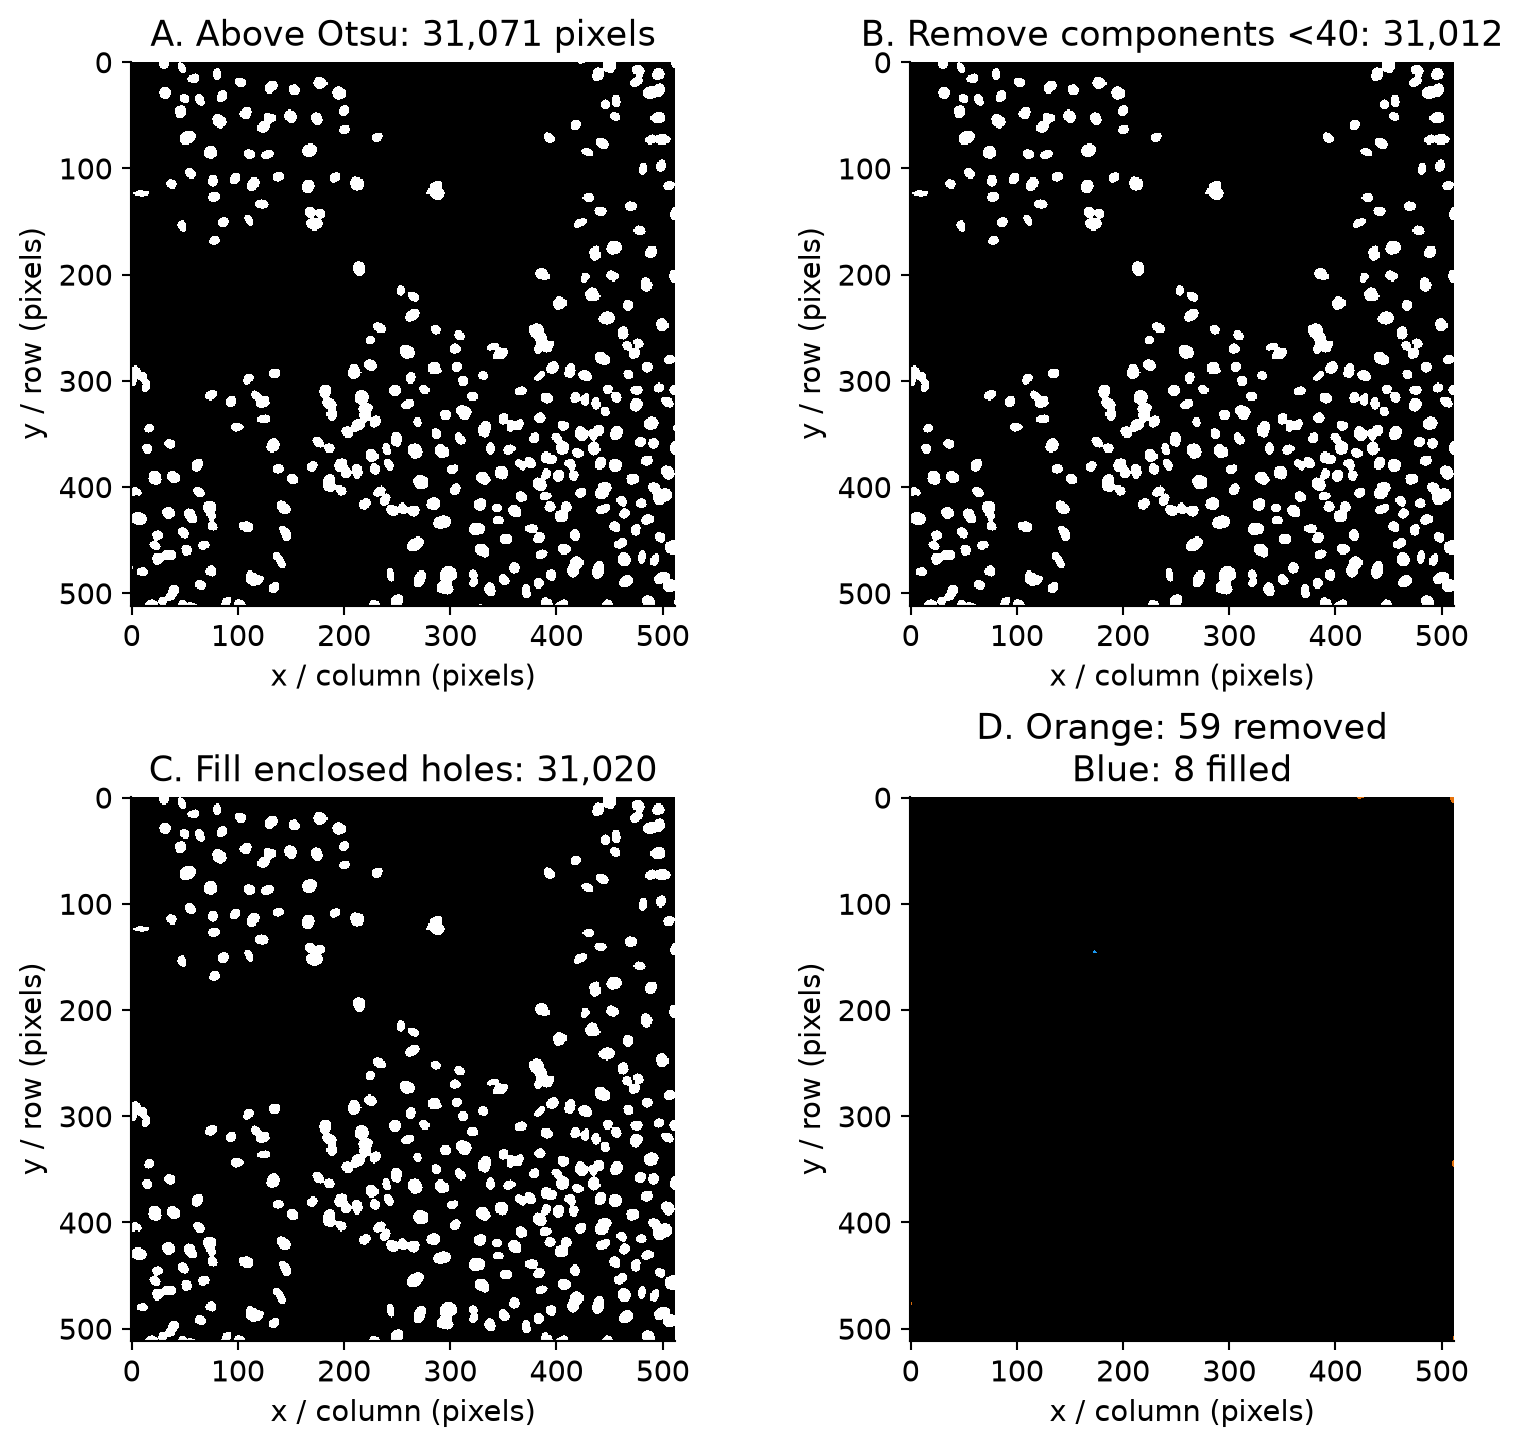
\includegraphics[width=0.94\linewidth]{09_mask_cleanup.png}
\caption{\diagnosticfig\ Mask construction and cleanup. A: 31,071 threshold-positive pixels. B: 31,012 pixels after excluding components smaller than 40\,\pxsq. C: 31,020 pixels after filling enclosed holes. D: changed pixels only; orange marks the 59 removed pixels and blue the eight filled pixels. The small visual difference reflects the small number of changed pixels.}
\label{fig:cleanup}
\end{figure}

\section{Step 5: fill enclosed holes in the foreground mask}
\label{sec:holes}

The next operation is:
\begin{lstlisting}[language=Python]
mask = ndi.binary_fill_holes(mask)
\end{lstlisting}
A hole is background that is enclosed by foreground and cannot be reached from the array boundary through the chosen background connectivity. Conceptually, the algorithm propagates through background from the outside; background it cannot reach is filled. With the default structure, background propagation is four-connected in two dimensions, using edge neighbours rather than diagonal steps.\cite{holes}

The notebook's introductory prose mentions ``small holes,'' but the implemented call has \textbf{no hole-size limit}. It fills all enclosed holes identified by that rule. The current input happens to add only eight pixels, taking the foreground total from 31,012 to 31,020.

This is different from smoothing the original image. No original grayscale value is replaced. Instead, some originally background-labelled pixels are assigned to the mask's foreground. Such a filled pixel can have a low raw intensity and need not individually satisfy the earlier intensity threshold. Once it belongs to a final region, it contributes to that region's area and raw-image intensity mean.

The biological assumption is that a dark interior opening should be included in the region's footprint. That may be reasonable for a solid object's silhouette and inappropriate for a true ring or cavity. The size and meaning of a hole should therefore be considered before applying this step to another microscopy problem.

\section{Step 6: compute a Euclidean distance transform}
\label{sec:distance}

The cleaned, filled mask supplies the geometry for separating touching structures:
\begin{lstlisting}[language=Python]
distance = ndi.distance_transform_edt(mask)
\end{lstlisting}
For a foreground pixel $x=(r,c)$, the distance transform gives the Euclidean distance to the nearest zero-valued background pixel:
\begin{equation}
D(x)=\min_{y\in\mathrm{background}}\|x-y\|_{2}.
\end{equation}
The transform is zero on background. Foreground pixels near the mask edge have small values, while pixels deep inside a broad foreground region have larger values. Default sampling is one unit per pixel along each axis, so the distances here are pixels.\cite{edt}

\begin{figure}[htbp]
\centering
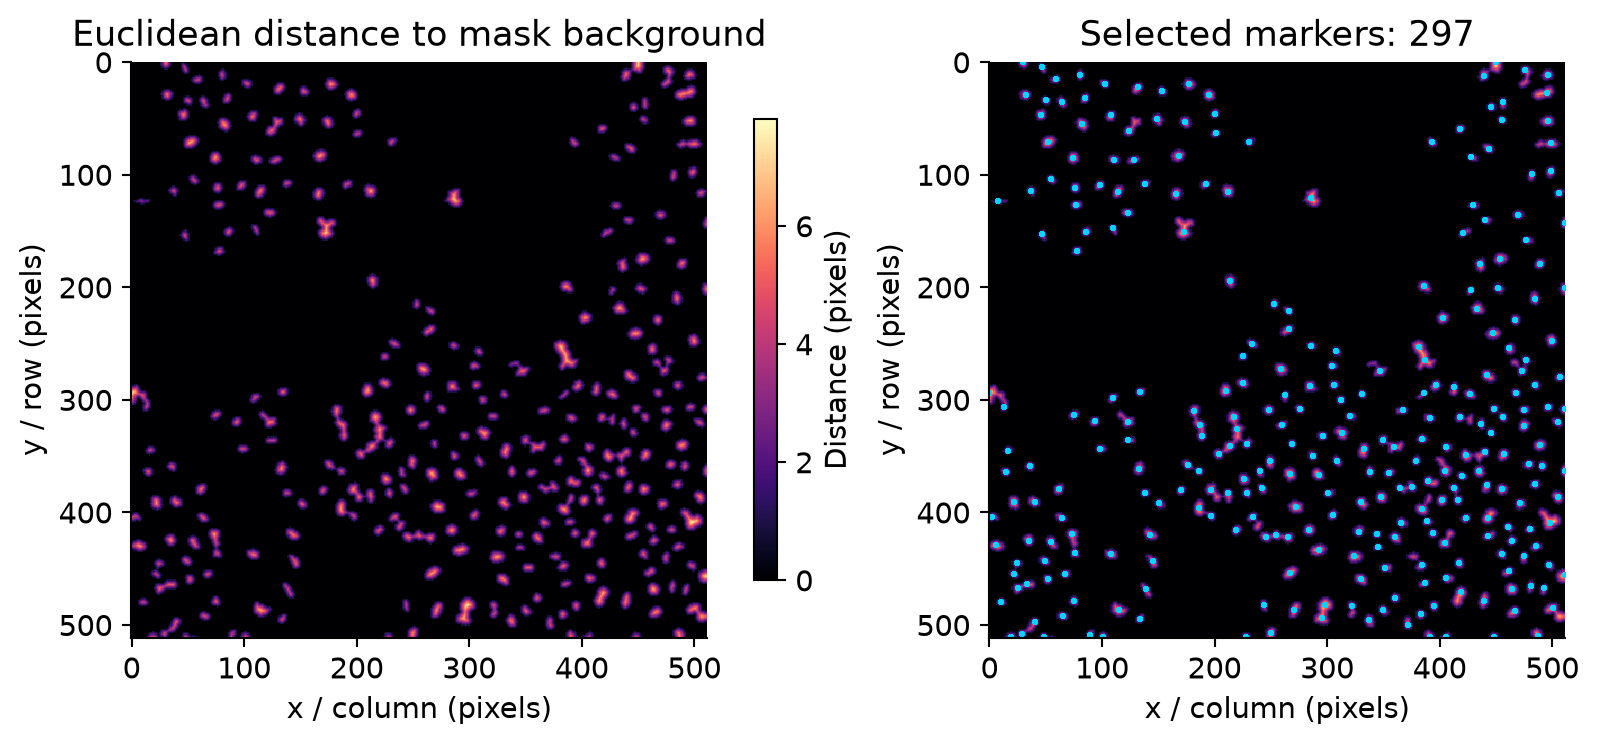
\includegraphics[width=\linewidth]{10_distance_seeds.png}
\caption{\diagnosticfig\ Left: Euclidean distance to the cleaned mask's background, with colour in pixel-distance units. Right: the same map with the selected seed positions in cyan. These bright distance centres are geometric features, not peaks in measured fluorescence.}
\label{fig:distance}
\end{figure}

The maximum distance is approximately 7.81 pixels in this reconstruction. The distance map is not a cell radius measurement or an intensity image. It is a representation of the already chosen foreground mask. If thresholding merges two objects with a narrow bridge, the merged mask can still have two thick interior centres, which motivates using distance peaks as separate starting points.

\section{Step 7: identify seed points and construct markers}
\label{sec:seeds}

The notebook chooses candidate centres and places an integer marker at each location:
\begin{lstlisting}[language=Python]
peaks = feature.peak_local_max(
    distance, min_distance=int(seed_spacing),
    labels=mask, exclude_border=False)
markers = np.zeros(image.shape, dtype=np.int32)
markers[tuple(peaks.T)] = np.arange(1, len(peaks) + 1)
\end{lstlisting}
The default seed spacing is eight pixels, and border peaks are permitted. The local-maximum search uses a square neighbourhood of side $2d+1$, which is $17\times17$ for $d=8$. Peak suppression uses the default Chebyshev, or maximum-coordinate, distance. This differs from the Euclidean distance used to create $D$.\cite{feature}

The parameter is a minimum-separation control for candidate seeds, not a measured cell diameter. A wider spacing can suppress nearby peaks; a narrower spacing can permit several seeds in one connected patch. Plateaus and equal-height candidates require a software tie-breaking rule and do not have an automatically privileged biological centre.

There is another implementation detail worth making explicit. The \field{labels=mask} argument receives a Boolean mask, so all foreground has the same nonzero label. The code does not first pass separately numbered connected components to the peak finder. Nearby disconnected foreground components can therefore influence peak suppression; a seed in every individual component is not guaranteed by this argument.

For the default image and parameters, 297 markers are selected. Their marker values 1 through 297 are identifiers assigned for computation, not biological categories or a time ordering. More seeds generally create more opportunities to split a region, but the final count also depends on coverage, watershed connectivity, and the later size filter.

\section{Step 8: partition the mask with marker-controlled watershed}
\label{sec:watershed}

\subsection{Why use negative distance?}
The central segmentation step is:
\begin{lstlisting}[language=Python]
labels = segmentation.watershed(-distance, markers, mask=mask)
\end{lstlisting}
Watershed treats an array as an elevation surface and grows regions from supplied markers. Using $-D$ turns thick foreground centres into low points or basins. Regions expand from the selected seeds within the Boolean mask until they meet competing regions. The mask prevents the procedure from flooding into the chosen background.\cite{segmentation}

This is a geometric partition of the foreground, not a learned cell-recognition model. Its effectiveness depends on whether the mask and marker positions correspond to the structures the researcher wants to distinguish. A single seed in a multi-lobed patch can leave it merged; too many seeds can split a plausible single object into several parts.

\subsection{Connectivity and boundary handling}
The watershed call's default \field{connectivity=1} uses four-neighbour propagation in two dimensions. The initial component filter used eight-neighbour connectivity, so the workflow is not uniformly eight-connected. A diagonally connected foreground configuration can behave differently at these two stages.

The defaults also include \field{compactness=0} and \field{watershed_line=False}. The algorithm does not deliberately insert zero-valued separator lines between adjacent basins. Distinct labels can meet directly along a boundary. Disconnected mask parts with no reachable marker can remain unlabelled in general; in the default reconstruction, all 31,020 filled-mask pixels receive a nonzero label.

\begin{figure}[htbp]
\centering
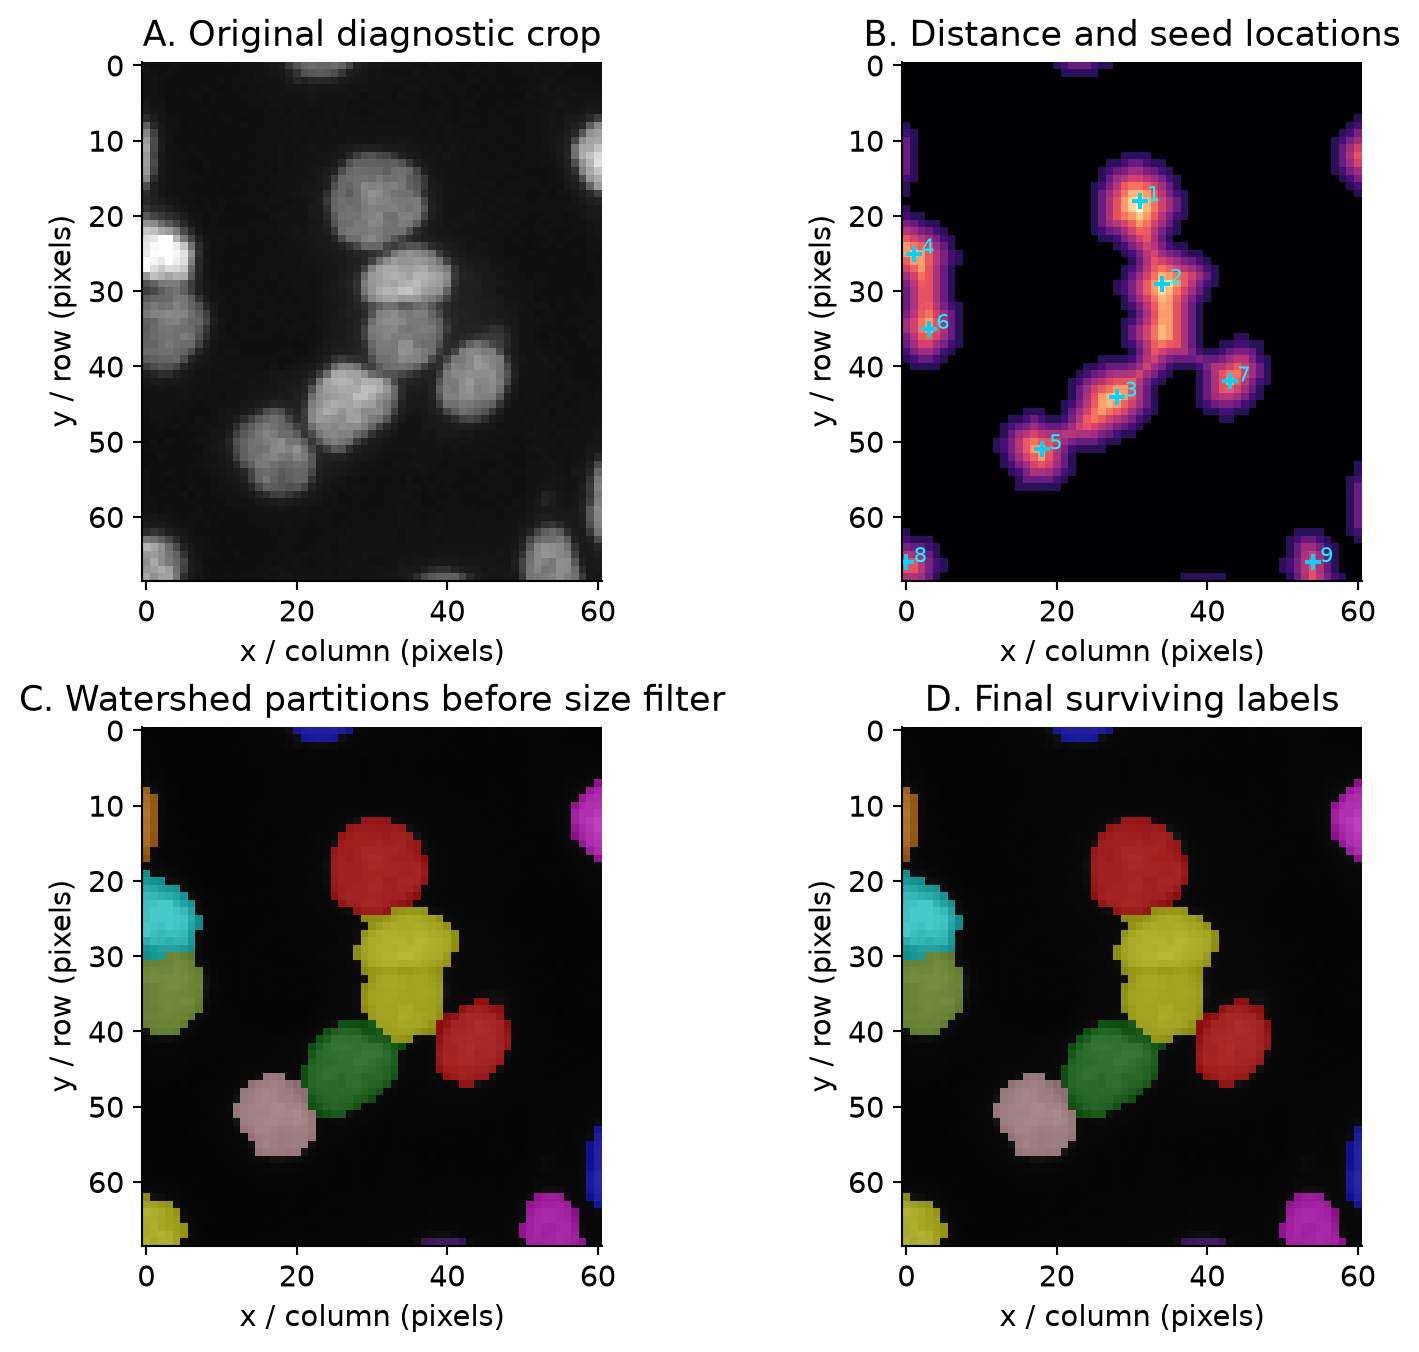
\includegraphics[width=0.94\linewidth]{11_watershed_crop.png}
\caption{\diagnosticfig\ A close view of the same diagnostic crop used for the Gaussian comparison. A: original intensities. B: distance values and numbered seed locations. C: watershed labels before the second area filter. D: final labels. Seed numbers are local annotations for this figure, not exported object IDs. Several labelled basins divide a connected group; whether they match biological objects requires human reference annotations.}
\label{fig:watershed}
\end{figure}

The default 269 retained connected components become 297 labelled regions, a net increase of 28 regions. This does not mean that exactly 28 components were split once each: individual components can generate different numbers of basins. The number records the partition produced by this marker configuration, rather than proving a number of cells.

\section{Step 9: apply the optional border policy}
\label{sec:border}

If the user selects \field{exclude_edges=True}, the code calls
\begin{lstlisting}[language=Python]
labels = segmentation.clear_border(labels)
\end{lstlisting}
after watershed. The default is False, so border-touching labels remain in the standard output and are flagged in the measurement table. When enabled, this operation removes entire labelled regions touching the full array boundary.\cite{segmentation}

The timing matters: it removes edge-touching watershed segments, not necessarily every segment originating from a connected component that once touched an edge. An interior segment split from that component can remain if its own label does not reach the border.

\begin{figure}[htbp]
\centering
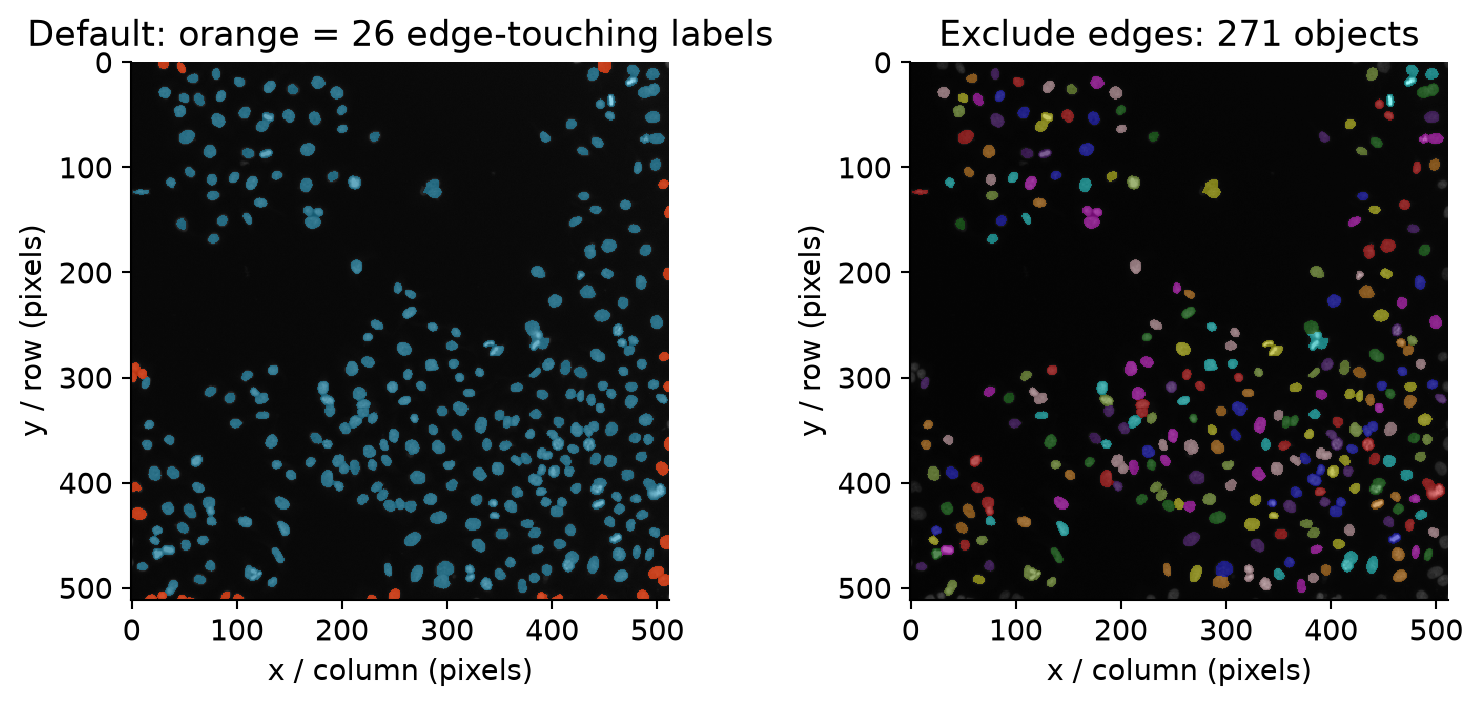
\includegraphics[width=\linewidth]{12_border_policy.png}
\caption{\diagnosticfig\ Left: default labels, with the 26 edge-touching objects highlighted in orange and other objects in blue. Right: a separate reconstruction with border exclusion enabled, retaining 271 objects. The colour categories in the left panel are deliberately defined for this diagnostic; they differ from the arbitrary label colours in the notebook overlays.}
\label{fig:border}
\end{figure}

Partial objects at an image boundary may have underestimated areas. Excluding them can be useful for shape measurements, but it also changes the sampled population and can introduce selection effects. Border exclusion does not automatically make an object-density estimate unbiased. The appropriate policy depends on the question and sampling design.

\section{Step 10: reapply the minimum area and relabel survivors}
\label{sec:postfilter}

Splitting can create small labelled regions even if their parent component was large enough to pass the initial area filter. The notebook therefore counts label pixels again and removes final segments smaller than 40\,\pxsq:
\begin{lstlisting}[language=Python]
sizes = np.bincount(labels.ravel())
keep = sizes >= int(min_area)
keep[0] = False
labels[~keep[labels]] = 0
labels, _, _ = segmentation.relabel_sequential(labels)
\end{lstlisting}
Discarded segment pixels become background; they are not redistributed to a neighbouring object. This is why final foreground coverage can vary with seed spacing even though the initial threshold mask is unchanged.

At the default settings, no post-watershed label is smaller than 40 pixels, so this second area check removes zero labels and zero pixels. Its inclusion is still meaningful for other parameter settings. The smallest surviving default object has 41 pixels; the criterion would have allowed 40, but no default output has exactly that size.

Sequential relabelling makes the surviving IDs consecutive. It helps indexing and export without changing the physical position of surviving pixels. An \field{object_id} is specific to one segmentation run; it is not a stable tracking identity across slider settings, crops, or images.

\section{Step 11: measure regions on the original image}
\label{sec:measurements}

\subsection{The mask supplies geometry; the original image supplies intensity}
The measurement loop uses
\begin{lstlisting}[language=Python]
for region in measure.regionprops(labels, intensity_image=image):
    # region.area, region.intensity_mean, region.centroid, region.bbox
\end{lstlisting}
The supplied intensity image is the original \field{uint8} array, not the Gaussian-smoothed array. This separates the image used to define the segmentation from the intensities measured inside its final regions.\cite{measure} It avoids silently replacing a reported raw mean by a smoothed-image mean, while retaining the dependence of each region's boundary on the preprocessing.

For region $R_j$, the exported area is
\begin{equation}
A_j=\sum_{(r,c)\in R_j}1,
\end{equation}
and its raw intensity mean is
\begin{equation}
\overline{I}_j=\frac{1}{A_j}\sum_{(r,c)\in R_j}I(r,c).
\end{equation}
The centroid is the unweighted mean of its pixel coordinates:
\begin{equation}
\overline{r}_j=\frac{1}{A_j}\sum_{(r,c)\in R_j}r,
\qquad
\overline{c}_j=\frac{1}{A_j}\sum_{(r,c)\in R_j}c.
\end{equation}
It is a geometric centroid, not an intensity-weighted bright centre. A bounding box is used to check whether a label reaches an image boundary; its upper row and column bounds are exclusive, which is why comparison with 512 correctly identifies the bottom or right edge.

\subsection{Output data dictionary}
\small
\begin{longtable}{L{0.26\linewidth}L{0.16\linewidth}L{0.49\linewidth}}
\caption{Columns in \field{objects.csv}. One row is one final labelled object.}\label{tab:dictionary}\\
\toprule
\textbf{Column} & \textbf{Unit / type} & \textbf{Meaning} \\
\midrule
\endfirsthead
\multicolumn{3}{l}{\textit{Table \thetable\ continued}}\\
\toprule
\textbf{Column} & \textbf{Unit / type} & \textbf{Meaning} \\
\midrule
\endhead
\bottomrule
\endfoot
\field{object_id} & Integer label & Sequential identifier within this run. It is unrelated to a biological type and is not stable across parameter changes. \\
\field{area_px2} & \pxsq & Number of pixels assigned to the final region. Without physical pixel calibration it cannot be reported in square micrometres. \\
\field{mean_intensity_0_255} & Raw 8-bit scale; floating mean & Mean of original image values in the final region, including any pixels admitted through hole filling. It is neither background-subtracted nor calibrated to molecule count. \\
\field{centroid_y_px} & Pixels; floating coordinate & Mean row coordinate. Rows increase downward in the displayed image; the full array uses row indices 0--511. \\
\field{centroid_x_px} & Pixels; floating coordinate & Mean column coordinate. Columns increase to the right. Centroids may be fractional because they average many integer coordinates. \\
\field{touches_edge} & Boolean & True if the final label's bounding box reaches any full-image boundary. A label merely touching the edge of a later display crop is not automatically an edge label in this table. \\
\end{longtable}
\normalsize

If pixel spacing $s_x$ and $s_y$ in micrometres were known, an area conversion would be $A_{\mu\mathrm{m}^{2}}=A_{\pxsq}s_xs_y$. Those spacings are not supplied here, so inserting a scale bar or a physical area would introduce unsupported information.

\subsection{What the saved default table contains}
The saved export has 297 rows with consecutive IDs and no missing fields. Areas range from 41 to 307\,\pxsq, with median 89 and mean 104.44\,\pxsq. Their sum is 31,020 pixels, or 11.8332\% of the full field. The size distribution is therefore a distribution of algorithm-defined regions from this one image, not a population estimate of cell size.

The per-object raw mean intensities range from 41.66 to 109.67. Their unweighted mean is 63.13; the area-weighted raw mean across all labelled pixels is 63.96. These statistics differ because giving every object equal weight differs from giving every included pixel equal weight. None is a direct test of segmentation accuracy.

\section{Step 12: read the final overlay and area histogram}
\label{sec:finalplots}

The notebook's three-panel plot should be read as a linked explanation:
\begin{enumerate}
  \item \textbf{Source image:} the unchanged grayscale field provides the evidence against which boundaries must be judged.
  \item \textbf{Coloured overlay:} colours distinguish segment labels. Transparency blends labels with the source image so a reader can inspect correspondence.\cite{colour} Colours do not identify cell types, treatments, or segmentation confidence, and the palette can repeat; colour alone is not a unique label identifier.
  \item \textbf{Object-size histogram:} 25 bins summarize final region areas. The minimum-area rule and segmentation choices partly determine its shape; it is not independent validation of those choices.
\end{enumerate}
The default figure reports 297 objects and a rounded threshold of 36.0. The selected bin width in the area histogram is a plotting choice. A visually concentrated size distribution does not establish that all regions correspond to the intended biological entities.

The full notebook plots are wide. The next page reproduces them in landscape orientation so the axes and original captions remain readable. The second plot uses factor 1.1 with the same minimum area and seed spacing; its computed cutoff is approximately 39.5457, displayed as 39.5.

\clearpage
\begin{landscape}
\begin{figure}[p]
\centering
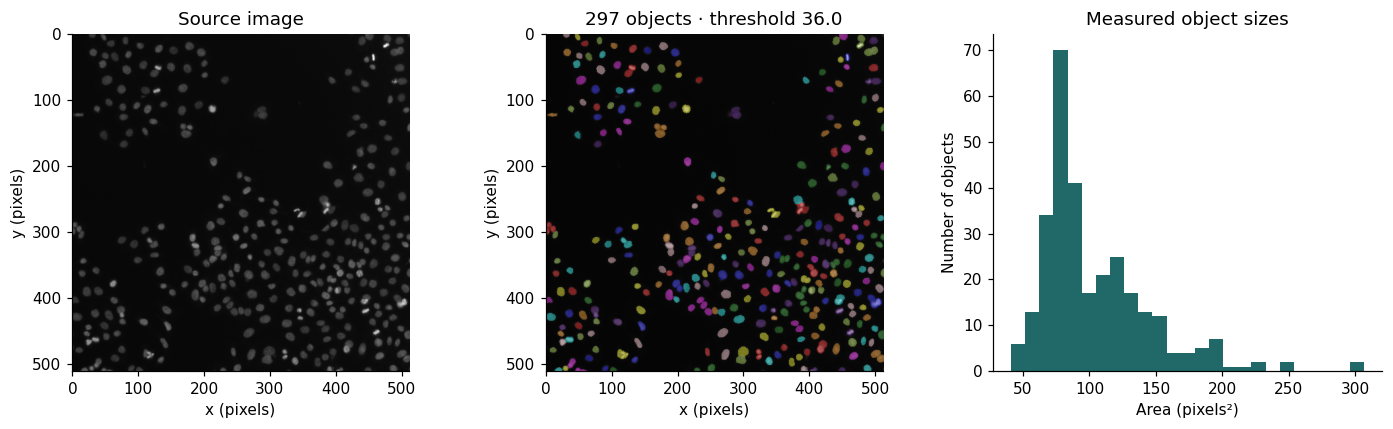
\includegraphics[width=0.94\linewidth]{02_notebook_default.png}
\caption{\notebookfig\ Default result: threshold factor 1.0, minimum area 40\,\pxsq, seed spacing 8 pixels, edge exclusion off. The title reports 297 objects. The notebook's stream output reports 26 edge-touching labels.}
\label{fig:default}
\vspace{6pt}
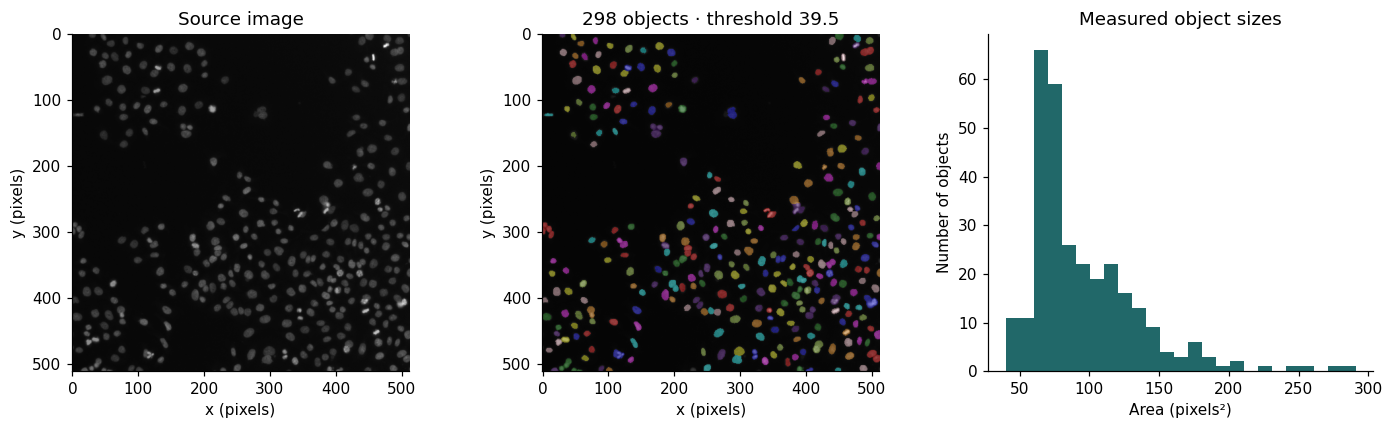
\includegraphics[width=0.94\linewidth]{03_notebook_threshold_1p1.png}
\caption{\notebookfig\ Stronger threshold, factor 1.1, with the other settings unchanged. The result contains 298 objects and 23 edge-touching labels. The increase in count despite a higher threshold illustrates that threshold-positive area and final object count are different quantities.}
\label{fig:thresholdhigher}
\end{figure}
\end{landscape}
\clearpage

\section{Step 13: change one control and assess sensitivity}
\label{sec:sensitivity}

\subsection{What the widgets change}
The sliders call the same \field{show_segmentation} and \field{segment_and_measure} functions that a user can call directly. They are an interface to explicit parameters, not a separate segmentation model.

\begin{table}[htbp]
\centering\small
\caption{Exposed controls in the notebook. Gaussian sigma, global Otsu selection, connectivity, and hole-filling behaviour remain fixed.}
\begin{tabularx}{\linewidth}{L{0.25\linewidth}L{0.20\linewidth}Y}
\toprule
\textbf{Control} & \textbf{Available values} & \textbf{What it changes} \\
\midrule
\field{threshold_factor} & 0.65--1.50, step 0.05; default 1.0 & Multiplies the Otsu cutoff before thresholding the smoothed image. \\
\field{min_area} & 10--200, step 10; default 40 & Sets the minimum component/region area used both before and after watershed. \\
\field{seed_spacing} & 3--20 pixels; default 8 & Controls local-maximum search and separation for distance-map seeds. \\
\field{exclude_edges} & False / True; default False & Keeps and flags, or removes, final watershed regions reaching the image boundary. \\
\bottomrule
\end{tabularx}
\end{table}

Continuous slider updates are disabled: the callback runs when a slider change is committed, reducing repeated recomputation during dragging. A direct function call is the portable alternative if the Jupyter frontend does not display widgets.

\subsection{Read the sensitivity heatmap as a dependence check}
The notebook deliberately varies threshold factor across 0.8, 1.0, and 1.2, and seed spacing across 5, 8, and 12 pixels, holding minimum area at 40. It reports object count, median area, and final labelled foreground percentage for the nine combinations.

\begin{figure}[htbp]
\centering
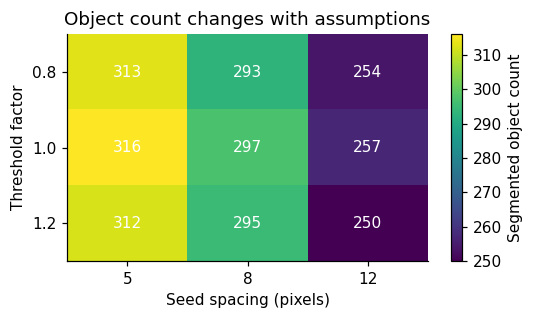
\includegraphics[width=0.78\linewidth]{04_notebook_sensitivity.png}
\caption{\notebookfig\ Final object count across nine parameter combinations. The heatmap measures parameter sensitivity. It does not compare the output with an independently annotated reference mask.}
\label{fig:sensitivity}
\end{figure}

\begin{table}[htbp]
\centering
\caption{The sensitivity values displayed by the notebook. Foreground percentage refers to surviving final labels, not the initial threshold mask.}
\label{tab:sensitivity}
\begin{tabular}{rrrrr}
\toprule
\textbf{Factor} & \textbf{Seed spacing, px} & \textbf{Objects} & \textbf{Median area, \pxsq} & \textbf{Foreground, \%} \\
\midrule
0.8 & 5 & 313 & 106 & 13.88 \\
0.8 & 8 & 293 & 108 & 13.90 \\
0.8 & 12 & 254 & 118 & 13.30 \\
1.0 & 5 & 316 & 87 & 11.83 \\
1.0 & 8 & 297 & 89 & 11.83 \\
1.0 & 12 & 257 & 99 & 11.23 \\
1.2 & 5 & 312 & 71 & 9.82 \\
1.2 & 8 & 295 & 73 & 9.86 \\
1.2 & 12 & 250 & 78 & 9.01 \\
\bottomrule
\end{tabular}
\end{table}

Several observations follow directly. Increasing the seed spacing to 12 gives fewer final objects in these tested cases. Increasing the threshold factor reduces median object area at a fixed seed spacing, but count is non-monotonic: at spacing 8, counts are 293, 297, and 295 for the three factors. In the separate factor-1.1 example, count is 298, one above the default despite a stronger threshold.

This behaviour is understandable because the pipeline changes topology as well as area. A stronger threshold can remove pixels, break a bridge, create a different seed configuration, or produce segments affected by the final area cutoff. Parameters interact, so counting more or fewer regions alone does not establish a better segmentation.

The nine-combination range of 250--316 objects is not a confidence interval for a true cell count. It summarizes a particular set of analysis choices. A stable result could still be systematically wrong, while an unstable result indicates that further definition and validation are needed.

\section{Step 14: inspect a crop and question the object definition}
\label{sec:crop}

The notebook next inspects rows 128:256 and columns 128:256. Python slices include the first index and exclude the second, so this is a 128-by-128 crop covering full-image indices 128--255 on both axes. Its displayed coordinates are local to the crop. Add 128 to a local row or column to recover the corresponding full-image coordinate.

\begin{figure}[htbp]
\centering
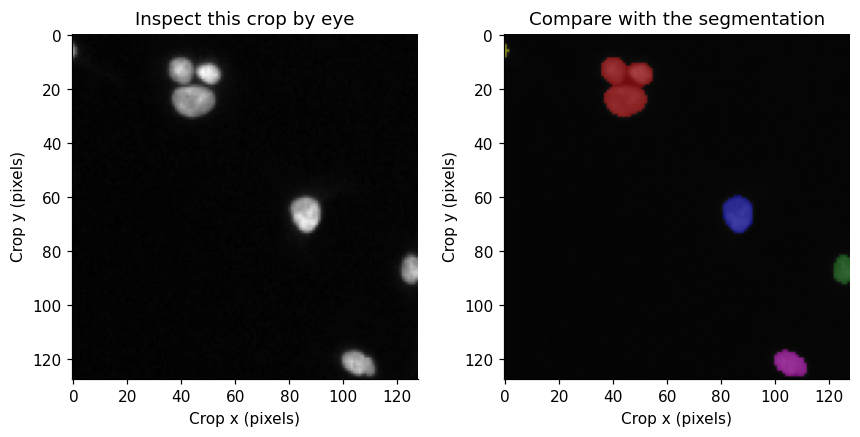
\includegraphics[width=\linewidth]{05_notebook_crop.png}
\caption{\notebookfig\ Original crop and segmentation overlay. The upper group of several bright lobes is displayed as one red label in the overlay. This is a concrete place to discuss a possible merge and the intended definition of an object. Biological correctness cannot be determined from the colour alone. The left grayscale panel autoscales to the crop's 7--108 range.}
\label{fig:crop}
\end{figure}

The crop contains parts of five exported labels, including partial regions intersecting the crop boundary. These are portions of objects measured from the full field; their area within the crop should not be substituted for their full exported area.

The upper multi-lobed structure makes the central judgment visible: should it count as one region or several biological entities? The algorithm has made a geometric decision based on this mask and its seeds. A researcher must first define the intended target before calling the result a merge or a correct single object. An independent reference annotation can then make the comparison meaningful.

Have two readers annotate the same crop, identify ambiguous cases, and agree on a rule before comparing the algorithm to a reference. The current notebook supplies a visual audit opportunity, not a validated reference mask. Metrics such as object detection precision/recall or mask intersection-over-union would require those annotations and a specified matching protocol; no such accuracy metric is calculated here.

\section{Step 15: export the result and preserve its provenance}
\label{sec:export}

The export cell explicitly constructs the default settings again:
\begin{lstlisting}[language=Python]
settings = {"threshold_factor": 1.0, "min_area": 40,
            "seed_spacing": 8, "exclude_edges": False}
labels, objects, threshold = segment_and_measure(**settings)
\end{lstlisting}
Consequently, exporting after moving a slider does not automatically save that slider's last view. The cell recomputes and saves the settings written in its dictionary. A user who wants another result should change and record those settings explicitly.

The outputs are:
\begin{itemize}
  \item \field{objects.csv}: one measurement row per final region;
  \item \field{segmentation.tif}: a 16-bit label image, where zero is background and positive integers identify objects;
  \item \field{settings.json}: source URL, image hash, parameter settings, actual intensity cutoff, recorded package versions, and interpretation note.
\end{itemize}
The label TIFF is a categorical region map. Its integer values are not fluorescence intensities; rendering it as though label 297 were brighter than label 1 would confuse identifiers with measurements.

The unchanged source TIFF has SHA-256:
\begin{quote}\small
\url{2751ba667c4067c5d30817cff004aa06f6f6287f1cdbb5b8c9c6a500308cb456}
\end{quote}
Saved settings identify NumPy 2.4.2, SciPy 1.17.0, scikit-image 0.26.0, and pandas 3.0.0 for the exported analysis. An independent reading of the saved label image reproduces every exported area, centroid, raw intensity mean, and edge flag. This checks consistency between those artifacts, not biological accuracy.

\section{What is established, and what still needs validation}

The example establishes how the specified software transforms this image into these regions. It provides inspectable parameters, an overlay, sensitivity results, a measurement table, and source identity. The default result is reproducible as an algorithmic calculation.

Further biological interpretation needs additional evidence. There is one microscopy field, not hundreds of independent biological replicates. Its 297 regions cannot be treated as 297 independent experiments. The source lacks the calibration needed for physical area, the reference mask needed for segmentation accuracy, and the biological annotations needed for a cell count or mitotic index.

Before using the method for a research claim, define the target object, obtain representative independent images, establish acquisition/calibration information, create or obtain reference annotations, and evaluate systematic misses, merges, splits, boundary errors, and parameter dependence. Background variation, intensity clipping, and acquisition differences should be assessed across the actual study images rather than inferred from this one example.

AI can help implement a requested control or explain a function, but it should preserve these definitions and limitations. A useful modification prompt asks for one replacement cell, states which parameters and measurements must remain unchanged, and requires observable checks. A plausible-looking overlay is the beginning of evaluation, not its completion.

\appendix
\section{Numerical ledger of the default pipeline}
\label{app:ledger}

The following intermediate values were reconstructed from the current function and original image for the supplemental diagnostics. The reconstructed final label array matches the saved \field{segmentation.tif} pixel-for-pixel. The ledger makes explicit which operations change the mask and which assign labels without changing default foreground coverage.

\small
\begin{longtable}{L{0.30\linewidth}L{0.16\linewidth}L{0.45\linewidth}}
\caption{Default pipeline ledger.}\label{tab:ledger}\\
\toprule
\textbf{Stage} & \textbf{Result} & \textbf{Interpretation} \\
\midrule
\endfirsthead
\multicolumn{3}{l}{\textit{Table \thetable\ continued}}\\
\toprule
\textbf{Stage} & \textbf{Result} & \textbf{Interpretation} \\
\midrule
\endhead
\bottomrule
\endfoot
Original image & 262,144 pixels & Intensities 7--255, median 10. \\
Gaussian smoothing & Range 7.452--225.234 & Floating-point intensity image; $\sigma=1$ pixel. \\
Otsu threshold & 35.95063855 & Computed on smoothed values; 256-bin histogram. \\
Threshold mask & 31,071 foreground pixels & Strict comparison above the default cutoff. \\
Initial connected components & 276 & Eight-connected foreground labelling. \\
Remove small components & 7 components; 59 pixels removed & Retain components with area at least 40 pixels. \\
Retained size-filtered mask & 269 components; 31,012 pixels & Some components still contain touching structures. \\
Fill holes & 8 pixels added & No size limit on enclosed holes. \\
Filled mask & 31,020 pixels & Supplies the geometry for the distance transform. \\
Distance transform & Maximum 7.810 pixels & Euclidean distance to zero-valued mask background. \\
Selected markers & 297 & Default peak spacing 8 pixels, border peaks allowed. \\
Watershed & 297 labels & Four-connected propagation; no unlabelled filled-mask pixels here. \\
Optional border removal & Off by default & Turning it on retains 271 objects in this example. \\
Final minimum-area check & 0 labels removed & Default segments all contain at least 40 pixels. \\
Sequential relabelling & IDs 1--297 & Identifiers within this run. \\
Final labelled area & 31,020 pixels; 11.8332\% & Area summed across surviving regions. \\
Object areas & 41--307\,\pxsq & Median 89; mean 104.44\,\pxsq. \\
Edge flags & 26 True; 271 False & Full-field boundary contact, not crop-boundary contact. \\
\end{longtable}
\normalsize

\section{Figure provenance and reproducibility of this report}
\label{app:provenance}

The five images marked \emph{Saved notebook figure} are the unchanged PNG payloads embedded in the saved notebook: intensity inspection, default segmentation, factor-1.1 segmentation, parameter-sensitivity heatmap, and visual-review crop. Their extraction does not rerun the notebook or regenerate its plots.

The saved execution counts are not monotonic: cells were run interactively and some were rerun later. The report therefore does not describe the retained plots as evidence of a single clean sequential kernel run. Their displayed default count, saved table, heatmap, and exported default mask are mutually consistent.

The seven images marked \emph{Supplemental diagnostic} were created for this report from the same source image and current algorithm: display scaling, Gaussian comparison, smoothed Otsu histogram, mask cleanup, distance/seed map, watershed crop, and border policy. The default trace was compared with both the saved label TIFF and the current function before those figures were authored. Its final labels match exactly.

Report generation executed the current segmentation function for default and border-excluded diagnostic comparisons and reconstructed its intermediate arrays. It did not rerun the entire notebook or overwrite its saved outputs.

The diagnostic environment used Python 3.11.6, NumPy 2.4.6, SciPy 1.17.1, scikit-image 0.26.0, pandas 3.0.6, and matplotlib 3.11.2. These patch versions differ from some versions recorded in the saved export. Both are documented rather than presented as one execution environment. The figures' filenames, extraction cells, saved execution counts, hashes, and diagnostic versions are retained in \field{microscopy_figures/figure_manifest.json}.

The figures and main \LaTeX{} file are bundled for Overleaf. Keep the \field{microscopy_figures} directory beside \field{microscopy_analysis_report.tex}; select the latter as the main document and use pdf\LaTeX{}. The original TIFF, CSV, label TIFF, Python environment, and notebook are not required to compile the report. The bibliography below is embedded in the source file.

\section{Plain-language glossary}
\begin{description}[style=nextline]
\item[Intensity] A pixel's stored grayscale value; its physical meaning requires acquisition/calibration information.
\item[Threshold] A cutoff that turns an intensity image into a foreground/background decision.
\item[Mask] A Boolean image describing which pixels are eligible for further processing.
\item[Connected component] A group of foreground pixels linked by a specified neighbourhood rule.
\item[Hole] An enclosed part of the mask's background that cannot be reached from the array boundary under the chosen connectivity.
\item[Distance transform] An image whose foreground values measure distance to the mask's background.
\item[Seed or marker] A selected starting position, given a label, from which a watershed region grows.
\item[Watershed] A method that partitions an allowed region into basins grown from supplied markers on an elevation-like array.
\item[Label image] An array in which each positive integer identifies an object; zero is background.
\item[Segmentation] The process of assigning image pixels to regions or objects.
\item[Sensitivity] How results change with analysis choices. It is distinct from accuracy against an independently established reference.
\end{description}

\clearpage
\addcontentsline{toc}{section}{References}
\begin{thebibliography}{9}
\bibitem{data}
scikit-image. \emph{Example data: human\_mitosis}. Image identity, source paper, and CC0 attribution to David Root.
\url{https://scikit-image.org/docs/0.26.x/api/skimage.data.html#skimage.data.human_mitosis}.
Reviewed October 24, 2026.
\bibitem{filters}
scikit-image. \emph{Filters API: gaussian and threshold\_otsu}. Parameters, numerical range handling, and histogram thresholding.
\url{https://scikit-image.org/docs/0.26.x/api/skimage.filters.html}.
Reviewed October 24, 2026.
\bibitem{gaussian}
SciPy. \emph{scipy.ndimage.gaussian\_filter}. Gaussian kernel truncation and boundary handling.
\url{https://docs.scipy.org/doc/scipy-1.17.0/reference/generated/scipy.ndimage.gaussian_filter.html}.
Reviewed October 24, 2026.
\bibitem{measure}
scikit-image. \emph{Measurement API: label and regionprops}. Connectivity, region geometry, raw intensity measurements, centroids, and bounding-box conventions.
\url{https://scikit-image.org/docs/0.26.x/api/skimage.measure.html}.
Reviewed October 24, 2026.
\bibitem{holes}
SciPy. \emph{scipy.ndimage.binary\_fill\_holes}. Background propagation and enclosed-hole filling.
\url{https://docs.scipy.org/doc/scipy-1.17.0/reference/generated/scipy.ndimage.binary_fill_holes.html}.
Reviewed October 24, 2026.
\bibitem{edt}
SciPy. \emph{scipy.ndimage.distance\_transform\_edt}. Exact Euclidean distance transform and pixel sampling convention.
\url{https://docs.scipy.org/doc/scipy-1.17.0/reference/generated/scipy.ndimage.distance_transform_edt.html}.
Reviewed October 24, 2026.
\bibitem{feature}
scikit-image. \emph{Feature API: peak\_local\_max}. Local-maximum footprint, spacing metric, labels, and boundary controls.
\url{https://scikit-image.org/docs/0.26.x/api/skimage.feature.html#skimage.feature.peak_local_max}.
Reviewed October 24, 2026.
\bibitem{segmentation}
scikit-image. \emph{Segmentation API: watershed, clear\_border, and relabel\_sequential}.
\url{https://scikit-image.org/docs/0.26.x/api/skimage.segmentation.html}.
Reviewed October 24, 2026.
\bibitem{colour}
scikit-image. \emph{Colour API: label2rgb}. Label overlays and display blending.
\url{https://scikit-image.org/docs/0.26.x/api/skimage.color.html#skimage.color.label2rgb}.
Reviewed October 24, 2026.
\end{thebibliography}
\end{document}
